\section{Nurul Izza Hamka | 1174062}
\subsection{Membaca Shapefile | PysHP}
\begin{enumerate}
 \item Nomor 1
 \lstinputlisting{src/tugas3/1174062/no1.py}
 \begin{figure}[H]
  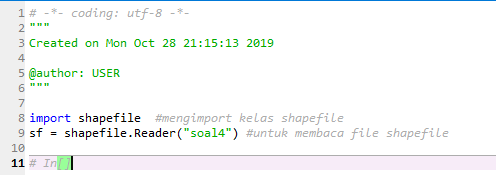
\includegraphics[width=6cm]{figures/Tugas3/1174062/Soal1.png}
  \centering
  \caption{Gambar Soal 1}
 \end{figure}
 \item Nomor 2
 \lstinputlisting{src/tugas3/1174062/no2.py}
 \begin{figure}[H]
  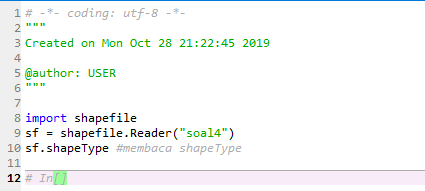
\includegraphics[width=6cm]{figures/Tugas3/1174062/Soal2.png}
  \centering
  \caption{Gambar Soal 2)}
 \end{figure}
 \item Nomor 3
 \lstinputlisting{src/tugas3/1174062/no3.py}
 \begin{figure}[H]
  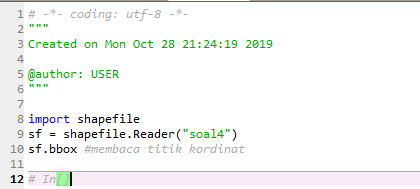
\includegraphics[width=6cm]{figures/Tugas3/1174062/Soal3.png}
  \centering
  \caption{Gambar Soal 3}
 \end{figure}
 \item Nomor 4
 \lstinputlisting{src/tugas3/1174062/no4.py}
 \begin{figure}[H]
  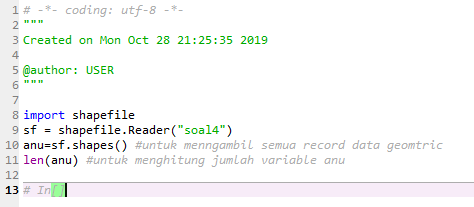
\includegraphics[width=6cm]{figures/Tugas3/1174062/Soal4.png}
  \centering
  \caption{Gambar Soal 4}
 \end{figure}
 \item Nomor 5
 \lstinputlisting{src/tugas3/1174062/no5.py}
 \begin{figure}[H]
  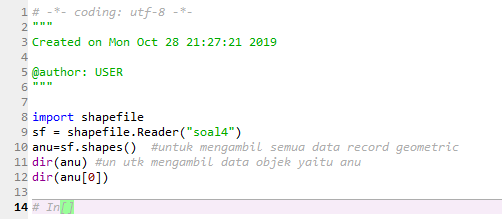
\includegraphics[width=6cm]{figures/Tugas3/1174062/Soal5.png}
  \centering
  \caption{Gambar Soal 5)}
 \end{figure}
 \item Nomor 6
 \lstinputlisting{src/tugas3/1174062/no6.py}
 \begin{figure}[H]
  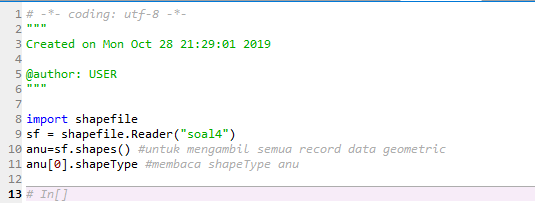
\includegraphics[width=6cm]{figures/Tugas3/1174062/Soal6.png}
  \centering
  \caption{Gambar Soal 6}
 \end{figure}
 \item Nomor 7
 \lstinputlisting{src/tugas3/1174062/no7.py}
 \begin{figure}[H]
  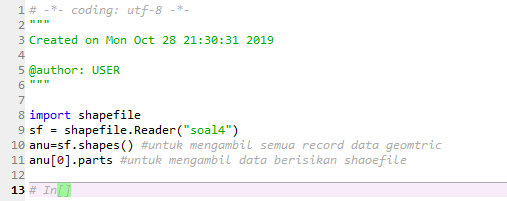
\includegraphics[width=6cm]{figures/Tugas3/1174062/Soal7.png}
  \centering
  \caption{Gambar Soal 7)}
 \end{figure}
 \item Nomor 8
 \lstinputlisting{src/tugas3/1174062/no8.py}
 \begin{figure}[H]
  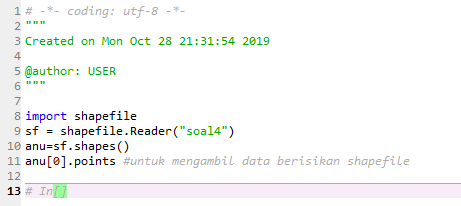
\includegraphics[width=6cm]{figures/Tugas3/1174062/Soal8.png}
  \centering
  \caption{Gambar Soal 8)}
 \end{figure}
 \item Nomor 9
 \lstinputlisting{src/tugas3/1174062/no9.py}
 \begin{figure}[H]
  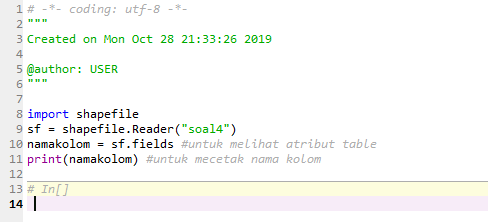
\includegraphics[width=6cm]{figures/Tugas3/1174062/Soal9.png}
  \centering
  \caption{Gambar Soal 9}
 \end{figure}
 \item Nomor 10
 \lstinputlisting{src/tugas3/1174062/no10.py}
 \begin{figure}[H]
  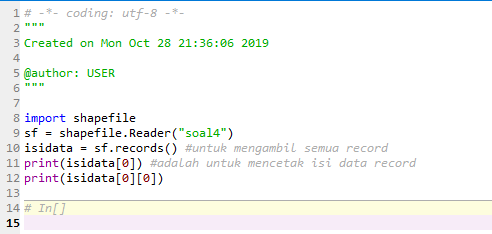
\includegraphics[width=6cm]{figures/Tugas3/1174062/Soal10.png}
  \centering
  \caption{Gambar Soal 10 }
 \end{figure}
 \item Nomor 11
 \lstinputlisting{src/tugas3/1174062/no11.py}
 \begin{figure}[H]
  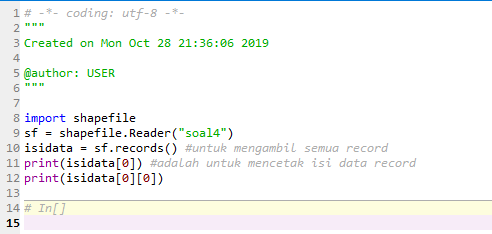
\includegraphics[width=6cm]{figures/Tugas3/1174062/Soal11.png}
  \centering
  \caption{Gambar Soal 11 }
 \end{figure}
\end{enumerate}
\subsection{Link}
https://youtu.be/IYd6ZhG4t6E